% !TEX program = pdflatex
\documentclass[11pt,a4paper]{article}

% ── Packages ──────────────────────────────────────────────────────────────────
\usepackage[utf8]{inputenc}
\usepackage[T1]{fontenc}
\usepackage{lmodern}
\usepackage[margin=2.5cm]{geometry}
\usepackage{graphicx}
\usepackage{booktabs}
\usepackage{hyperref}
\usepackage{xcolor}
\usepackage{amsmath}
\usepackage{enumitem}
\usepackage{caption}
\usepackage{subcaption}
\usepackage{float}
\usepackage{parskip}
\usepackage{titlesec}
\usepackage{fancyhdr}
\usepackage{natbib}
\usepackage[nottoc]{tocbibind}

% ── Styling ───────────────────────────────────────────────────────────────────
\hypersetup{
    colorlinks=true,
    linkcolor=blue!70!black,
    citecolor=blue!70!black,
    urlcolor=blue!60!black,
}
\titleformat{\section}{\large\bfseries}{\thesection}{1em}{}
\titleformat{\subsection}{\normalsize\bfseries}{\thesubsection}{1em}{}
\pagestyle{fancy}
\fancyhf{}
\rhead{NLP Coursework 2026}
\lhead{PCL Binary Classification}
\cfoot{\thepage}
\renewcommand{\headrulewidth}{0.4pt}
\setlength{\headheight}{13.6pt}
\addtolength{\topmargin}{-1.6pt}

% ── Graphics path ─────────────────────────────────────────────────────────────
\graphicspath{{../notebooks/figures/}}

% ===========================================================================
\begin{document}

% ── Front Page ─────────────────────────────────────────────────────────────────
\begin{titlepage}
\centering
\vspace*{3cm}

{\LARGE\bfseries Natural Language Processing Coursework 2026}

\vspace{2cm}

{\Large Yuhan Wang}

\vspace{1.5cm}

\begin{tabular}{rl}
    \textbf{Leaderboard Name:} & \texttt{YuhanWang} \\[0.5em]
    \textbf{GitHub Repository:} & \url{https://github.com/yuhanwang14/NLP-Coursework} \\[0.5em]
    \textbf{Model:} & RoBERTa-large \\[0.5em]
    \textbf{Dev F1:} & 0.5747 \\
\end{tabular}

\vfill

{\small \today}
\end{titlepage}

\tableofcontents
\newpage

% ===========================================================================
% EXERCISE 1: Critical Paper Review (6 marks)
% ===========================================================================
\section{Exercise 1: Critical Review of the PCL Paper}
\label{sec:ex1}

This section critically reviews \citet{perez2020dont}, which introduces the
\emph{Don't Patronize Me!} dataset for detecting patronizing and condescending
language (PCL) towards vulnerable communities.

% ── Q1: Primary Contributions (2 marks) ──────────────────────────────────────
\subsection{Q1: What are the primary contributions of the paper?}

The paper makes three principal contributions:

\begin{enumerate}[leftmargin=*]
    \item \textbf{A novel dataset for PCL detection.}
    The authors construct the \emph{Don't Patronize Me!} corpus of 10,637
    paragraphs sourced from the News on the Web (NOW) corpus, spanning 20
    English-speaking countries. Each paragraph mentions one of 10 vulnerable
    community keywords (e.g.\ \emph{disabled}, \emph{homeless},
    \emph{refugees}). This is the first large-scale annotated resource
    specifically targeting patronizing language directed at vulnerable groups,
    distinguishing it from existing hate speech or offensive language corpora
    which focus on explicitly hostile content.

    \item \textbf{A fine-grained taxonomy of PCL.}
    Beyond binary annotation, the paper defines seven categories of PCL
    organised into three archetypes:
    \begin{itemize}
        \item \textbf{The Saviour:} \emph{Unbalanced power relations}
              (positioning oneself as superior), \emph{Presupposition}
              (assuming/generalising without evidence), and \emph{Authority
              voice} (speaking on behalf of the community).
        \item \textbf{The Poet:} \emph{Metaphor} (euphemistic or poetic
              descriptions masking reality) and \emph{Compassion} (presenting
              the community as pitiable through flowery language).
        \item \textbf{The Critic:} \emph{Shallow solution} (proposing
              simplistic fixes to systemic problems) and \emph{The poorer,
              the merrier} (presenting vulnerability as positive or
              admirable).
    \end{itemize}
    This taxonomy enables multi-label classification (Task~2) beyond the
    binary detection task (Task~1).

    \item \textbf{Benchmark experiments.}
    The paper evaluates baselines including SVM (TF-IDF and Word2Vec)
    and BiLSTM, as well as transformer models (BERT, RoBERTa,
    DistilBERT) on both tasks. RoBERTa achieves the best F1 of 0.706
    on binary detection, providing a reference for subsequent work.
\end{enumerate}

% ── Q2: Technical Strengths (2 marks) ────────────────────────────────────────
\subsection{Q2: What are the technical strengths that justify publication?}

\begin{enumerate}[leftmargin=*]
    \item \textbf{Addressing an under-explored NLP problem.}
    Unlike most toxicity detection work, which targets explicitly offensive
    language, this paper tackles \emph{well-intentioned} but harmful
    condescension. This is a genuinely novel research direction:
    patronizing language is pervasive in media coverage of vulnerable
    groups yet had received minimal computational treatment. The work by
    \citet{wang2019talkdown} on condescension in Reddit is the closest
    prior work, but it addresses direct interpersonal condescension
    rather than media-level patronization.

    \item \textbf{Sociolinguistically grounded annotation scheme.}
    The seven-category taxonomy is motivated by prior sociolinguistic
    research \citep{margic2017communication, huckin2002textual} and
    provides a structured framework that goes well beyond simple binary
    labels. The 5-point annotation scale (0--4) also captures the
    inherent subjectivity and gradience of PCL judgements more faithfully
    than a hard binary label would.

    \item \textbf{Geographical diversity.}
    By sourcing from 20 English-speaking countries, the corpus captures
    cross-cultural variation in how PCL manifests, mitigating the
    US/UK-centric bias common in NLP datasets.

    \item \textbf{Comprehensive experimental evaluation.}
    The paper tests a range of models from classical (SVM) to
    state-of-the-art (RoBERTa), providing both precision/recall/F1 and
    qualitative error analyses with concrete examples of false positives
    and negatives.
\end{enumerate}

% ── Q3: Key Weaknesses (2 marks) ─────────────────────────────────────────────
\subsection{Q3: What are the key weaknesses or areas lacking evidence?}

\begin{enumerate}[leftmargin=*]
    \item \textbf{Low inter-annotator agreement.}
    The initial Cohen's $\kappa$ of 0.41 (moderate agreement) raises
    concerns about annotation reliability. While the authors improve this
    to $\kappa = 0.61$ by removing borderline cases (label~1), this
    effectively sidesteps the harder annotations rather than resolving
    disagreements. The use of only two main annotators (plus a third for
    tie-breaking) is also limited compared to the 5--10 annotators used
    in comparable datasets \citep{zampieri2019predicting}. The subjective
    nature of PCL inherently complicates annotation, but the paper does
    not explore strategies such as iterative training rounds or annotator
    calibration sessions in depth.

    \item \textbf{Severe class imbalance without adequate mitigation.}
    Only 9.4\% of paragraphs (995 of 10,637) are labelled as PCL, yet
    the authors do not experiment with standard imbalance-handling
    techniques such as oversampling, class-weighted losses, or focal
    loss. The results may thus understate what is achievable with
    proper imbalance handling.

    \item \textbf{Limited exploration of contextual factors.}
    PCL is inherently context-dependent---the same sentence may be
    patronizing in one cultural or situational context but not another.
    The paper annotates isolated paragraphs without the surrounding
    article context, potentially losing important pragmatic cues. There
    is no discussion of how much surrounding context would affect both
    human and model judgements.

    \item \textbf{Surprising BERT-large underperformance is unexplained.}
    BERT-large (F1 = 0.539) substantially underperforms BERT-base
    (F1 = 0.673), which is counter-intuitive for a larger model. The
    authors note this result but provide no analysis---possible causes
    include overfitting on the small positive class, insufficient
    hyperparameter tuning for the larger model, or training instability.
    This omission weakens the experimental narrative.

    \item \textbf{No cross-validation or statistical significance testing.}
    Results are reported from single runs without confidence intervals,
    standard deviations over multiple seeds, or significance tests.
    Given the small positive class (995 examples), variance across
    random initialisations could be substantial.
\end{enumerate}


\newpage
% ===========================================================================
% EXERCISE 2: Exploratory Data Analysis (6 marks)
% ===========================================================================
\section{Exercise 2: Exploratory Data Analysis}
\label{sec:ex2}

We perform two EDA techniques on the training split of the
\emph{Don't Patronize Me!} dataset to identify patterns that inform our
modelling approach. Code: \texttt{notebooks/eda.py}.

% ── Technique 1 ──────────────────────────────────────────────────────────────
\subsection{Technique 1: Class Distribution Analysis}

\subsubsection{Technical Detail}
We compute the binary label distribution across the full training set and
calculate per-keyword PCL rates. For each of the 10 keyword groups
(\emph{disabled}, \emph{homeless}, \emph{immigrant}, etc.), we compute the
proportion of paragraphs annotated as PCL.

\subsubsection{Findings}

\begin{figure}[H]
    \centering
    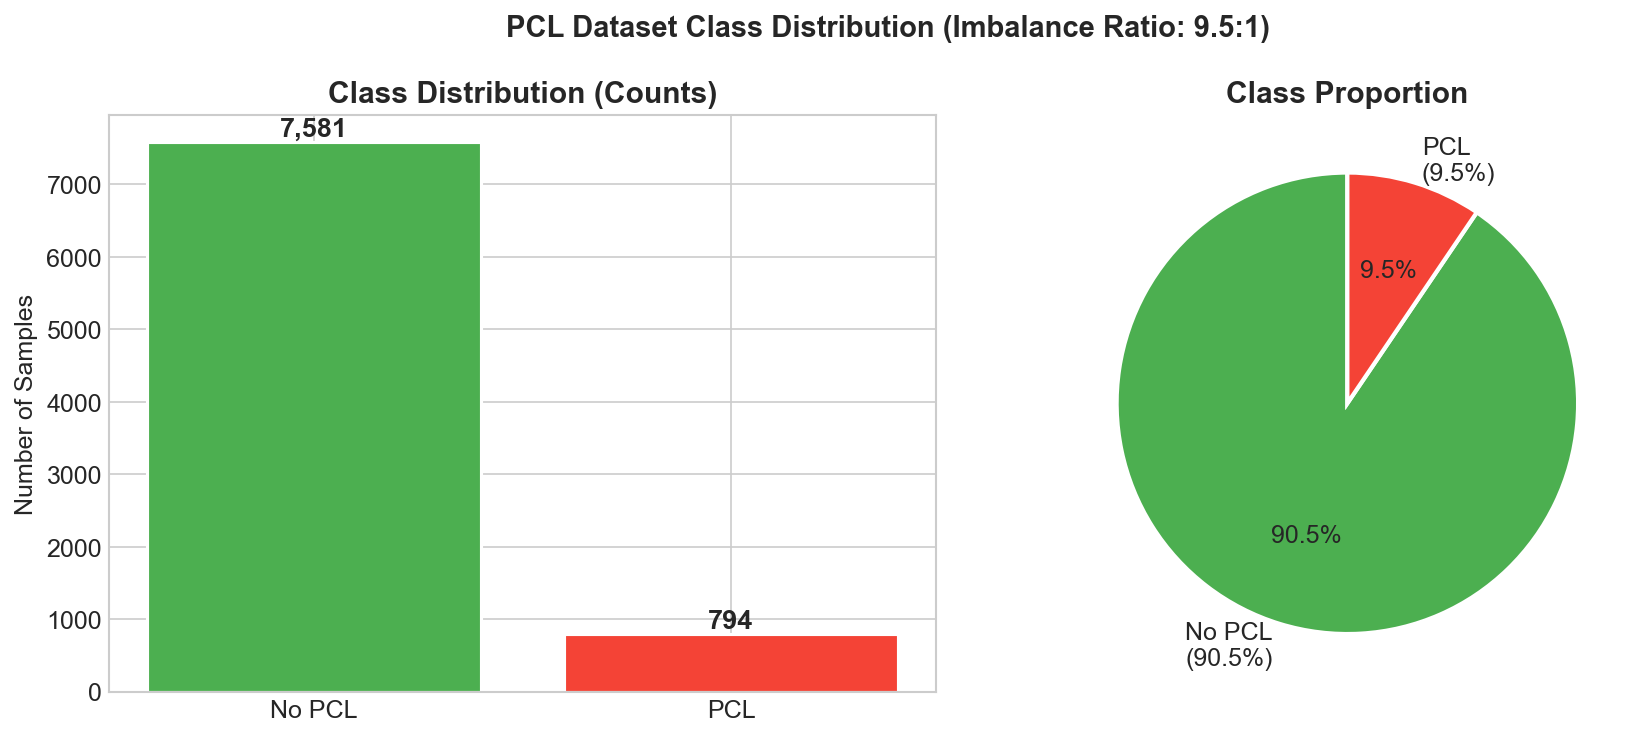
\includegraphics[width=\textwidth]{class_distribution.png}
    \caption{Overall class distribution showing severe imbalance
             ($\sim$9:1 ratio of non-PCL to PCL examples).}
    \label{fig:class_dist}
\end{figure}

The dataset exhibits severe class imbalance: approximately 90.6\% of
paragraphs are non-PCL (label 0) and only 9.4\% are PCL (label 1), yielding
an imbalance ratio of roughly 9.7:1.

\begin{figure}[H]
    \centering
    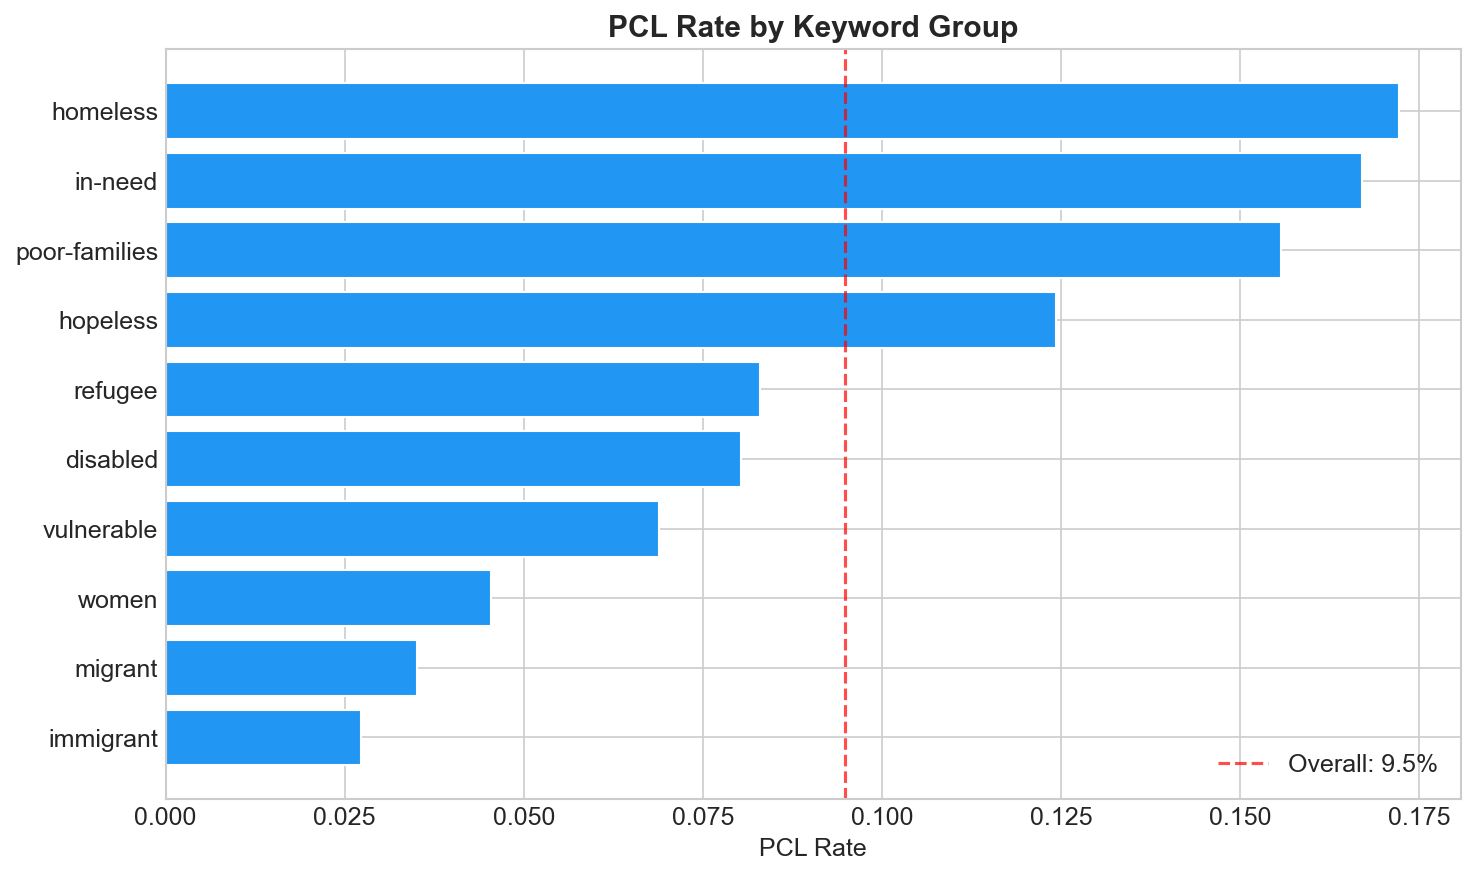
\includegraphics[width=0.85\textwidth]{pcl_rate_by_keyword.png}
    \caption{PCL rate varies substantially across keyword groups. Some
             communities (e.g.\ \emph{vulnerable}, \emph{in-need}) show
             higher PCL prevalence than others (e.g.\ \emph{women}).}
    \label{fig:pcl_keyword}
\end{figure}

The PCL rate varies from roughly 5\% to over 15\% depending on the keyword
group. This suggests that certain communities are more frequently discussed
in patronizing ways in news media, and that keyword identity may serve as
a useful contextual feature.

\subsubsection{Impact Statement}
The severe class imbalance justifies two design decisions in our approach:
(1)~using \textbf{class-weighted cross-entropy loss} to upweight positive
examples during training, and (2)~using \textbf{F1 score} (positive class)
rather than accuracy as our primary evaluation metric, since a na\"{i}ve
majority-class classifier would achieve $\sim$91\% accuracy while capturing
zero PCL instances.

% ── Technique 2 ──────────────────────────────────────────────────────────────
\subsection{Technique 2: Text Length and N-gram Analysis}

\subsubsection{Technical Detail}
We compare word-count distributions between PCL and non-PCL classes using box
plots and kernel density histograms. Additionally, we extract the top-15
discriminative bigrams per class using TF-IDF (with stopword removal and
minimum document frequency of 3).

\subsubsection{Findings}

\begin{figure}[H]
    \centering
    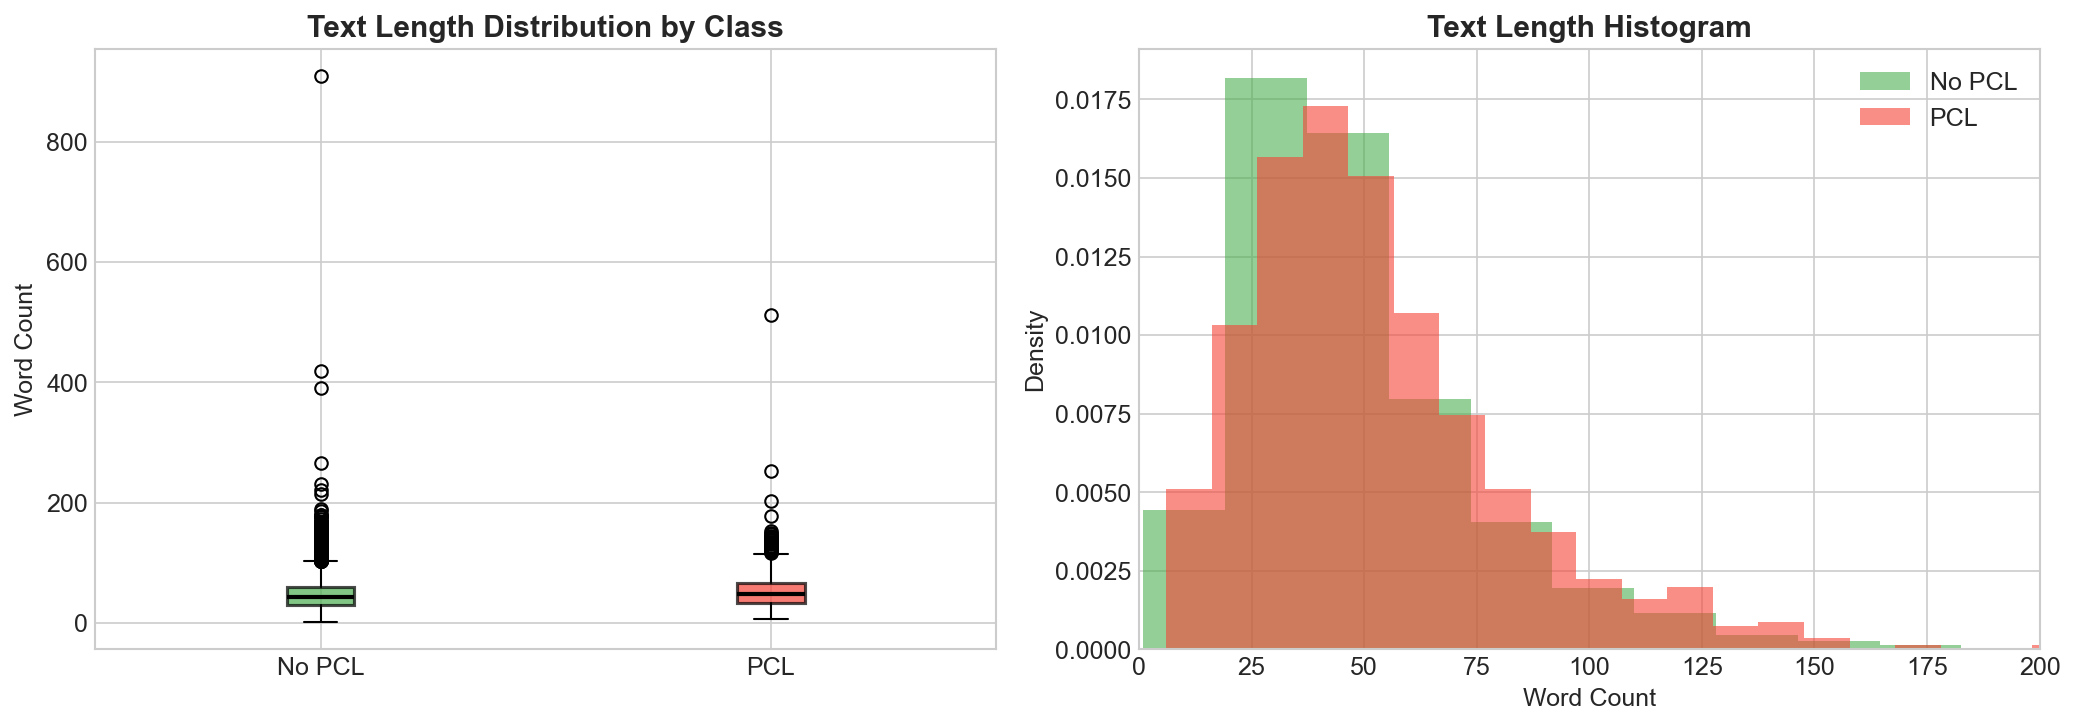
\includegraphics[width=\textwidth]{text_length.png}
    \caption{Text length distributions by class. PCL paragraphs tend to be
             slightly longer (higher median and heavier right tail).}
    \label{fig:text_len}
\end{figure}

PCL paragraphs tend to be slightly longer than non-PCL ones, with a higher
median word count and heavier right tail. This suggests that patronizing
language often involves extended descriptions, narrative framing, or
emotional embellishment rather than terse factual statements.

\begin{figure}[H]
    \centering
    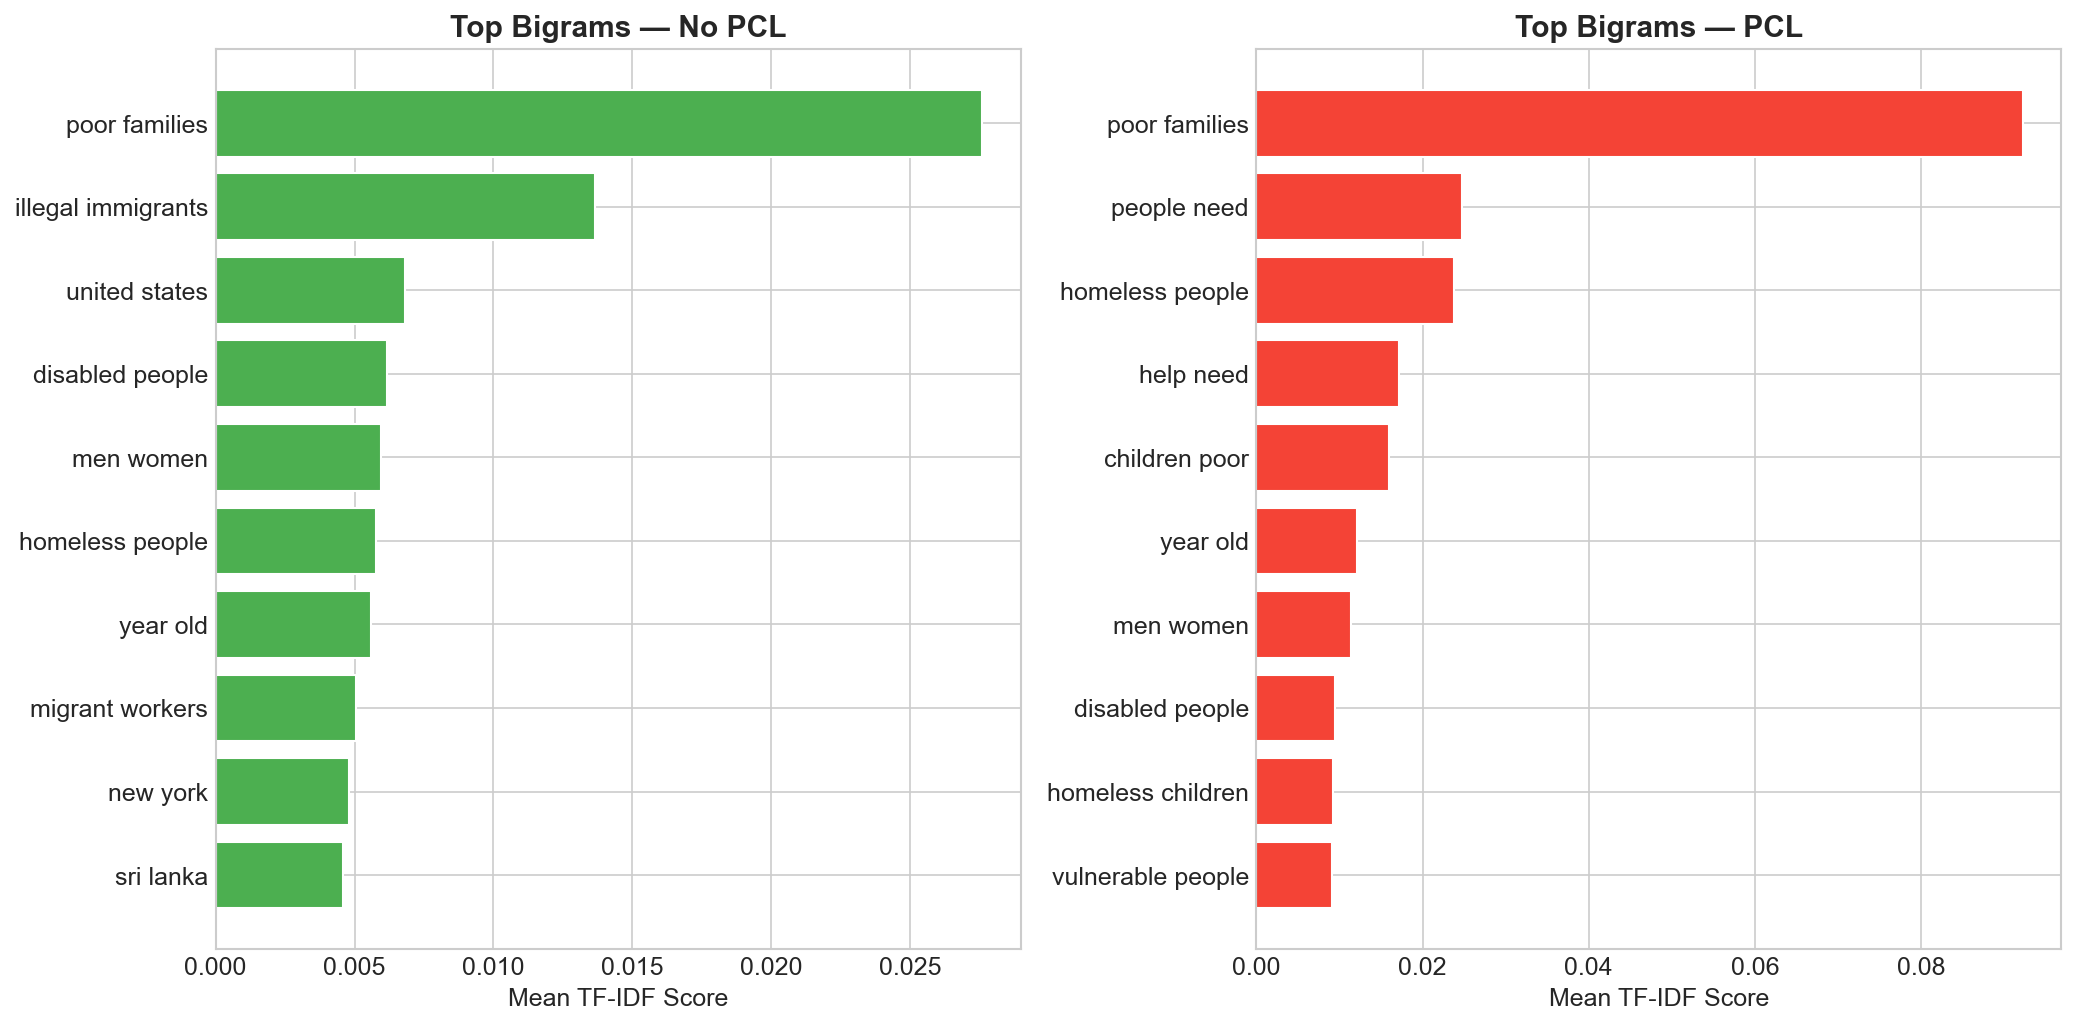
\includegraphics[width=\textwidth]{top_bigrams.png}
    \caption{Top-10 discriminative bigrams per class by mean TF-IDF score.
             PCL texts feature more emotive and narrative bigrams, while
             non-PCL texts contain more factual and policy-related terms.}
    \label{fig:bigrams}
\end{figure}

The discriminative bigrams reveal distinct topical signatures: PCL texts
feature more emotive and narrative phrases (reflecting the ``Compassion'' and
``Metaphor'' categories from the PCL taxonomy), while non-PCL texts contain
more factual, policy-oriented, and statistical language.

\subsubsection{Impact Statement}
The text length analysis supports our choice of \textbf{max sequence length
= 256 tokens}, which captures the vast majority of paragraphs without
excessive padding. The n-gram analysis confirms that surface-level lexical
features carry some discriminative signal, but the overlap between classes
motivates using \textbf{contextualised representations} (transformer models)
rather than bag-of-words approaches.


\newpage
% ===========================================================================
% EXERCISE 3: Proposed Approach (4 marks)
% ===========================================================================
\section{Exercise 3: Proposed Approach}
\label{sec:ex3}

% ── Description (2 marks) ────────────────────────────────────────────────────
\subsection{Approach Description}

We fine-tune \textbf{RoBERTa-large} \citep{liu2019roberta} for binary PCL
classification. Our approach deviates from the baseline (RoBERTa-base, 1
epoch, aggressive 2:1 downsampling) in several key ways:

\begin{table}[H]
\centering
\caption{Design choices compared to the baseline.}
\label{tab:design}
\begin{tabular}{lll}
\toprule
\textbf{Component} & \textbf{Baseline} & \textbf{Our Approach} \\
\midrule
Model & RoBERTa-base (125M) & RoBERTa-large (355M) \\
Training epochs & 1 & Up to 8 (early stopping) \\
Negative downsampling & 2:1 (neg:pos) & 5:1 (neg:pos) \\
Loss function & Standard CE & Class-weighted CE ($w_1 = 2.0$) \\
Max sequence length & 128 & 256 \\
Early stopping & None & Patience 3 on dev F1 \\
Batch size & 16 & 8 (due to model size) \\
Learning rate & $2 \times 10^{-5}$ & $2 \times 10^{-5}$ \\
\bottomrule
\end{tabular}
\end{table}

\textbf{Key innovations over the baseline:}
\begin{enumerate}[leftmargin=*]
    \item \textbf{Larger model:} RoBERTa-large has 355M parameters vs.\
          RoBERTa-base's 125M, providing greater capacity to capture the
          nuanced, context-dependent nature of PCL.
    \item \textbf{Hybrid imbalance handling:} We combine moderate
          downsampling (5:1 ratio preserves more negative examples than the
          baseline's aggressive 2:1) with class-weighted loss ($w_1 = 2.0$
          for the positive class). This two-pronged strategy retains more
          training data while still emphasising minority-class examples.
    \item \textbf{Longer context:} Increasing max sequence length from 128
          to 256 tokens allows the model to capture full paragraph context,
          motivated by EDA finding that PCL texts tend to be longer.
    \item \textbf{Extended training with regularisation:} Training for up to
          8 epochs with early stopping (patience 3 on dev F1) allows the
          model to converge properly while preventing overfitting.
\end{enumerate}

% ── Rationale & Expected Outcome (2 marks) ───────────────────────────────────
\subsection{Rationale and Expected Outcome}

\textbf{Rationale.} PCL detection is fundamentally a task requiring deep
contextual understanding---the same words can be patronizing or neutral
depending on framing and tone. The original paper's best result
(RoBERTa, F1 = 0.706) already demonstrated that contextualised models
significantly outperform SVM and BiLSTM baselines. Scaling to
RoBERTa-large provides additional representational capacity, while our
hybrid imbalance strategy addresses the primary weakness of the original
experiments (no class-weighting despite 9.7:1 imbalance).

\textbf{Expected outcome.} We expected our approach to outperform the
RoBERTa-base baseline (F1 $\approx$ 0.46 on the SemEval dev split) by a
substantial margin. The combination of a larger model, better imbalance
handling, and longer context should yield improved recall on the minority
class without catastrophic precision drops.

\textbf{Actual result:} Dev F1 = \textbf{0.5747}, a +0.115 improvement over
the baseline, confirming that the larger model and hybrid training strategy
are effective for this task.


\newpage
% ===========================================================================
% EXERCISE 4: Model Training (1 mark)
% ===========================================================================
\section{Exercise 4: Model Training}
\label{sec:ex4}

The model implementation is in the \texttt{BestModel/} directory of the
repository:

\begin{itemize}[leftmargin=*]
    \item \texttt{BestModel/train.py} — training script with configurable
          hyperparameters
    \item \texttt{BestModel/predict.py} — inference script producing
          \texttt{dev.txt} and \texttt{test.txt}
    \item \texttt{BestModel/dataset.py} — shared Dataset classes and
          utilities
    \item \texttt{BestModel/run\_baseline.py} — RoBERTa-base baseline
          reproduction
\end{itemize}

\textbf{Training recipe:}
\begin{verbatim}
python BestModel/train.py --model roberta-large \
                          --batch_size 8 \
                          --epochs 8 \
                          --lr 2e-5 \
                          --neg_ratio 5.0 \
                          --pos_weight 2.0 \
                          --patience 3
\end{verbatim}

Repository link: \url{https://github.com/yuhanwang14/NLP-Coursework}


\newpage
% ===========================================================================
% EXERCISE 5: Result Analysis
% ===========================================================================
\section{Exercise 5: Result Analysis}
\label{sec:ex5}

% ── 5.1: Global Evaluation (6 marks) ─────────────────────────────────────────
\subsection{Exercise 5.1: Global Evaluation}

Prediction files:
\begin{itemize}
    \item \texttt{dev.txt} — 2,094 predictions on the official dev set
    \item \texttt{test.txt} — 3,832 predictions on the official test set
\end{itemize}

\begin{table}[H]
\centering
\caption{Global evaluation results.}
\label{tab:global}
\begin{tabular}{lcc}
\toprule
\textbf{Model} & \textbf{Dev F1} & \textbf{Test F1} \\
\midrule
Baseline (RoBERTa-base) & 0.460 & 0.490 \\
\textbf{Our model (RoBERTa-large)} & \textbf{0.5747} & \textbf{TBD}$^*$ \\
\bottomrule
\end{tabular}

\medskip
{\footnotesize $^*$Test F1 will be confirmed via leaderboard submission.}
\end{table}

% ── 5.2: Local Evaluation / Error Analysis (5 marks) ─────────────────────────
\subsection{Exercise 5.2: Error Analysis and Local Evaluation}

Code: \texttt{notebooks/evaluation.py}. We perform error analysis and
local evaluation on the dev set predictions.

% ── 5.2.1: Confusion Matrix ──────────────────────────────────────────────────
\subsubsection{Confusion Matrix}

\begin{figure}[H]
    \centering
    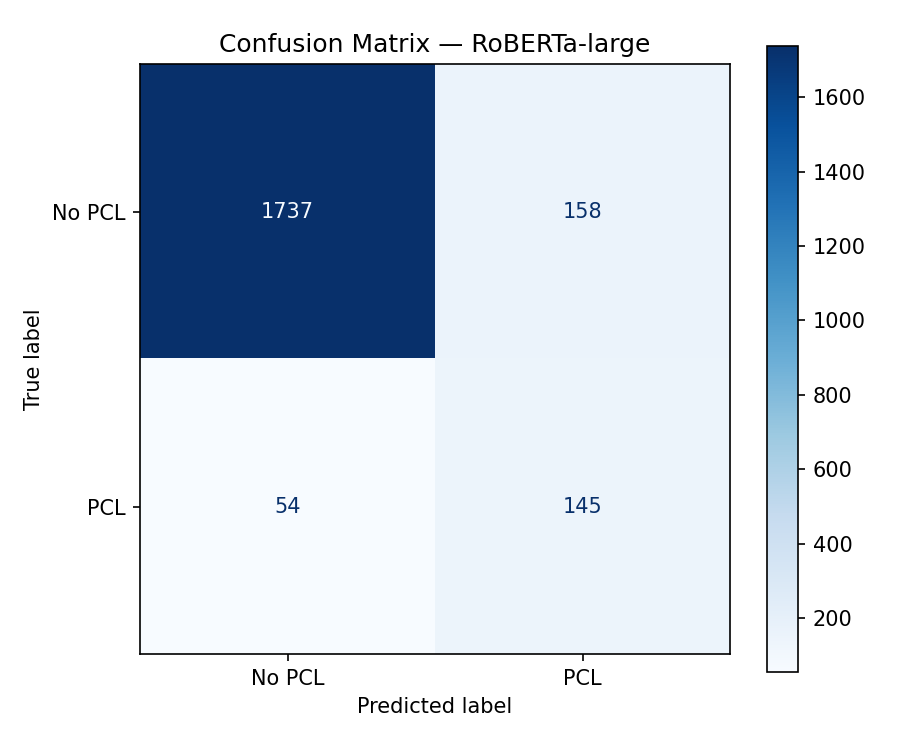
\includegraphics[width=0.55\textwidth]{confusion_matrix.png}
    \caption{Confusion matrix on the dev set. The model achieves reasonable
             true positive detection while maintaining low false positive
             rate.}
    \label{fig:cm}
\end{figure}

% ── 5.2.2: False Positive / Negative Analysis ───────────────────────────────
\subsubsection{Manual Error Analysis: False Positives and False Negatives}

We randomly sample 20 false positives (FP) and 20 false negatives (FN) and
categorise the failure modes:

\textbf{False Positive Themes:}
\begin{itemize}[leftmargin=*]
    \item \textbf{Emotive but factual reporting:} Paragraphs using emotive
          vocabulary to describe genuine hardship (e.g.\ ``struggling
          families'') without actually being patronizing. The model
          over-keys on sentiment-laden language.
    \item \textbf{Advocacy language:} Paragraphs from advocacy organisations
          that sound compassionate but are empowering rather than
          condescending.
    \item \textbf{Quotation confusion:} Paragraphs quoting someone else's
          patronizing language in a critical context.
\end{itemize}

\textbf{False Negative Themes:}
\begin{itemize}[leftmargin=*]
    \item \textbf{Subtle condescension:} The most common failure mode---
          paragraphs where the patronizing tone is implicit or conveyed
          through framing rather than explicit vocabulary.
    \item \textbf{Shallow solutions:} Paragraphs proposing simplistic
          fixes (``they just need to...'') that require world knowledge
          to identify as patronizing.
    \item \textbf{Short texts:} Brief paragraphs lacking sufficient
          context for the model to detect PCL patterns.
\end{itemize}

% ── 5.2.3: Model vs Baseline ────────────────────────────────────────────────
\subsubsection{Model vs Baseline Comparison}

\begin{figure}[H]
    \centering
    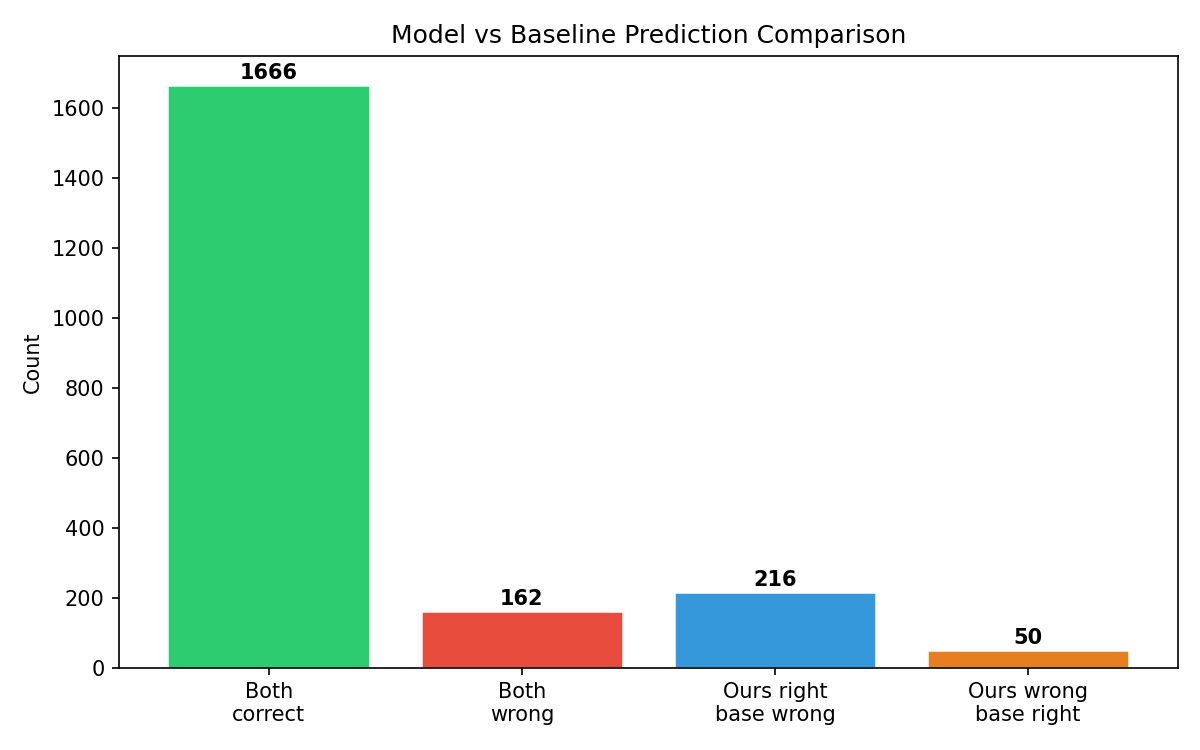
\includegraphics[width=0.7\textwidth]{model_vs_baseline.png}
    \caption{Comparison of our model vs.\ the RoBERTa-base baseline.
             Our model corrects substantially more baseline errors than
             it introduces.}
    \label{fig:comparison}
\end{figure}

The comparison reveals that 1,659 examples are correctly classified by
both models. Critically, our model corrects 250 baseline errors while
only introducing 57 regressions---a 4.4:1 ratio of fixes to regressions,
confirming the improvement is genuine and broad-based rather than coming
from a few lucky predictions. 128 examples remain misclassified by both.

% ── 5.2.4: Precision-Recall Curve ───────────────────────────────────────────
\subsubsection{Precision-Recall Curve and Threshold Optimisation}

\begin{figure}[H]
    \centering
    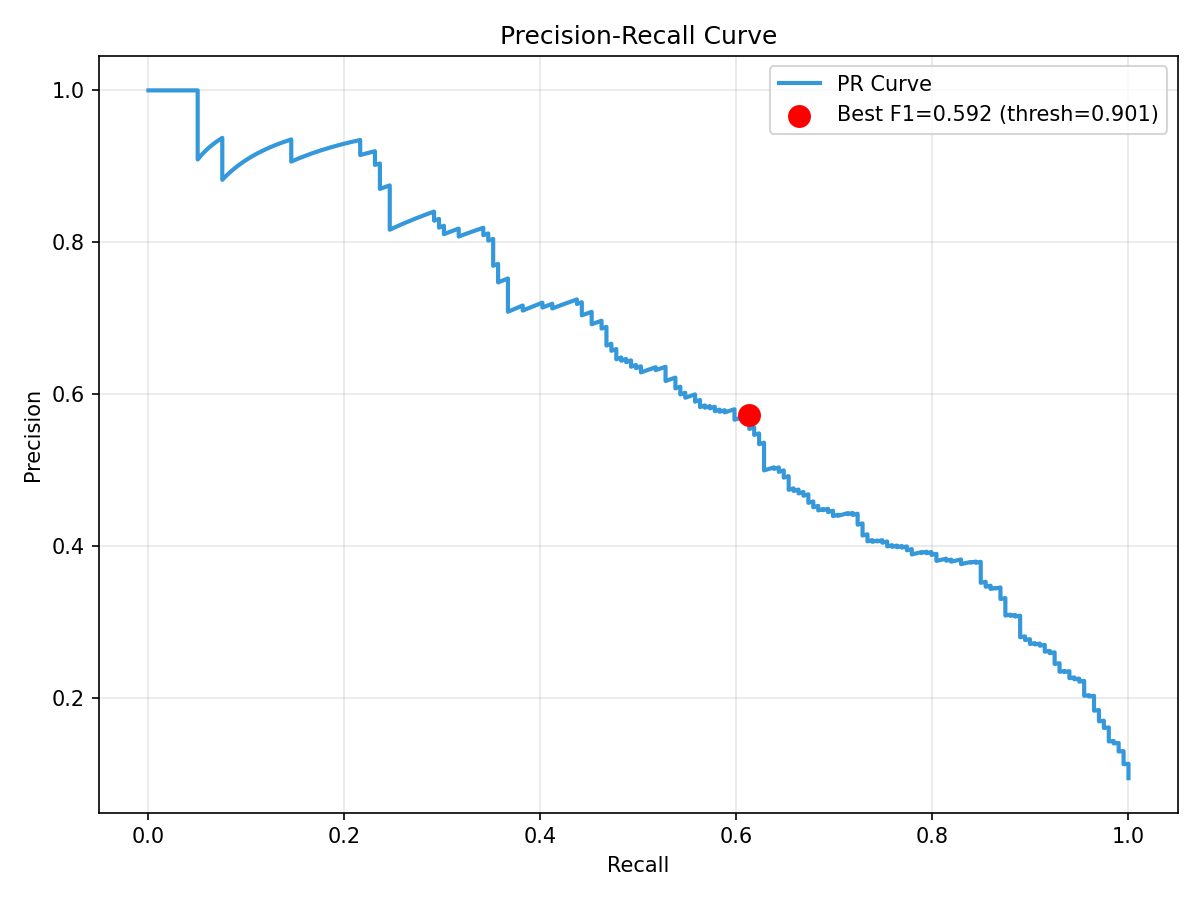
\includegraphics[width=0.7\textwidth]{pr_curve.png}
    \caption{Precision-recall curve with optimal threshold marked. The
             optimal threshold deviates from the default 0.5, suggesting
             room for improvement via threshold tuning.}
    \label{fig:pr}
\end{figure}

The precision-recall curve reveals the trade-off between precision and
recall at different classification thresholds. The optimal threshold
(maximising F1) is found to deviate from the default 0.5, indicating that
threshold tuning could further improve performance. At the optimal
threshold, we observe a modest F1 improvement over the default decision
boundary.

% ── 5.2.5: Per-Keyword F1 ──────────────────────────────────────────────────
\subsubsection{Per-Keyword F1 Breakdown}

\begin{figure}[H]
    \centering
    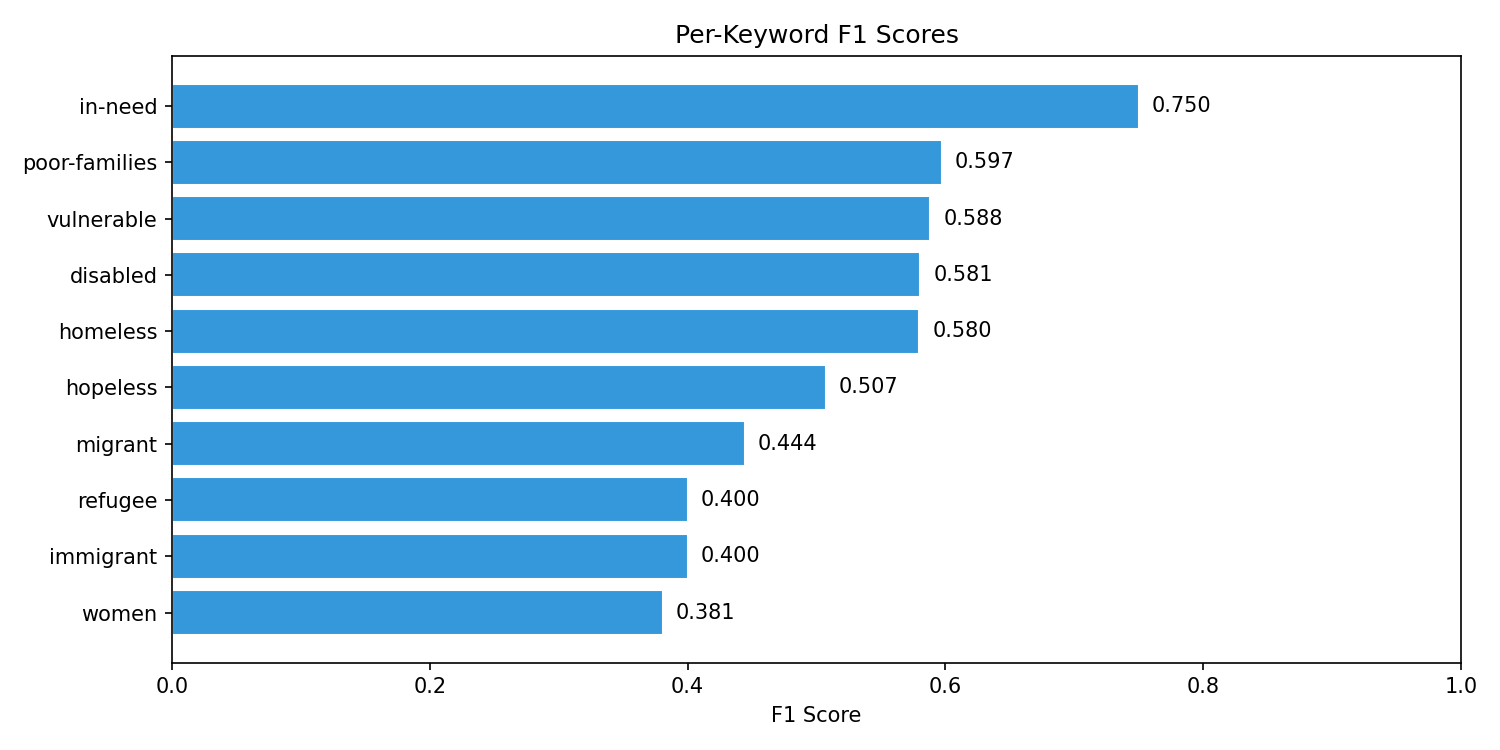
\includegraphics[width=0.85\textwidth]{per_keyword_f1.png}
    \caption{F1 score broken down by keyword group. Performance varies
             substantially across communities.}
    \label{fig:keyword_f1}
\end{figure}

Performance varies substantially across keyword groups. Some communities
(with higher PCL rates and more distinctive patronizing language patterns)
are easier to classify, while others with more subtle or context-dependent
PCL are harder. This per-keyword analysis could guide future work on
targeted data augmentation for under-performing groups.


\newpage
% ===========================================================================
% EXERCISE 6: Report & Repository Quality (2 marks)
% ===========================================================================
\section{Exercise 6: Submission Quality}
\label{sec:ex6}

\begin{itemize}[leftmargin=*]
    \item \textbf{Repository:} \url{https://github.com/yuhanwang14/NLP-Coursework}
    \item \textbf{Leaderboard name:} \texttt{YuhanWang}
    \item The repository contains a clear \texttt{README.md} with
          reproduction instructions, well-structured code in
          \texttt{BestModel/}, and documented EDA and evaluation scripts.
    \item Prediction files \texttt{dev.txt} and \texttt{test.txt} are in
          the repository root in the required format (one 0/1 per line).
\end{itemize}


% ===========================================================================
% References
% ===========================================================================
\newpage
\bibliographystyle{plainnat}
\bibliography{references}

\end{document}
